%class
	\documentclass{beamer}

%template
	\usetheme{HannoverSalman}
	\setbeamertemplate{navigation symbols}{}
	%\setbeamertemplate{footline}{\centering{\insertframenumber/\insertpresentationendpage}}
	%\setbeamertemplate{footline}{\hspace*{.5cm}\scriptsize{\hfill\insertframenumber\hspace*{.5cm}}} 


%packages
	\usepackage{amsmath, amssymb, graphicx,cancel}
	\usepackage[absolute,overlay]{textpos}
	\usepackage{subfigure}
	\usepackage{caption}\captionsetup{labelformat=empty,labelsep=none}
	\usepackage{geometry}
	\geometry{verbose}
	\usepackage{color}
	\usepackage{xmpmulti}
	\usepackage[3D]{movie15}
	\usepackage{hyperref}
%	\usepackage{bookmark}
	\usepackage[open,openlevel=4,atend]{bookmark}
	%\bookmarksetup{color=blue}
	\usepackage{multirow}
	\usepackage[style=numeric,defernumbers, authoryear]{biblatex}
	%\usepackage[square,sort]{natbib}
	%\usepackage{fancyhdr}%\pagestyle{fancy} 

	
	\hypersetup{bookmarksdepth = 4}


%citations files
	\bibliography{MyCitations}

%logoCSIPCPL
    \setlength{\TPHorizModule}{1mm}
    \setlength{\TPVertModule}{1mm}
    \newcommand{\logoCSIPCPL}
    {
    	\begin{textblock}{1}(100,2) %(100,85)  for bottom
    		
\includegraphics[width=1.5cm]{figs/logo_CSIP}
    	\end{textblock}
    	
	\begin{textblock}{1}(117,1) %(117,85)  for bottom
    		
\includegraphics[width=1.0cm]{figs/logo_CPL}
    	\end{textblock} 
    }

%logo evolution
    \newcommand{\logoEvolution}
    {    	
	\begin{textblock}{1}(110,1) %(117,85)  for bottom
    		\includegraphics[width=0.65in]{figs/logo_evolution.pdf}
    	\end{textblock} 
    }

%logo Qualcomm
    \newcommand{\logoQualcomm}
    {
    	\begin{textblock}{1}(110,2) %(100,85)  for bottom
    		\includegraphics[width=1.5cm]{figs/logo_qualcomm.jpg}
    	\end{textblock}
    }
%logo Qualcomm (long)
    \newcommand{\logoQualcommllong}
    {
    	\begin{textblock}{1}(0,0) 
    		\includegraphics[width=1.25in]{figs/logo_qualcomm_long.jpg}
    	\end{textblock}
    }

%logo Tech Tower
    \newcommand{\logoTechTower}
    {
    	\begin{textblock}{1}(0,0) 
    		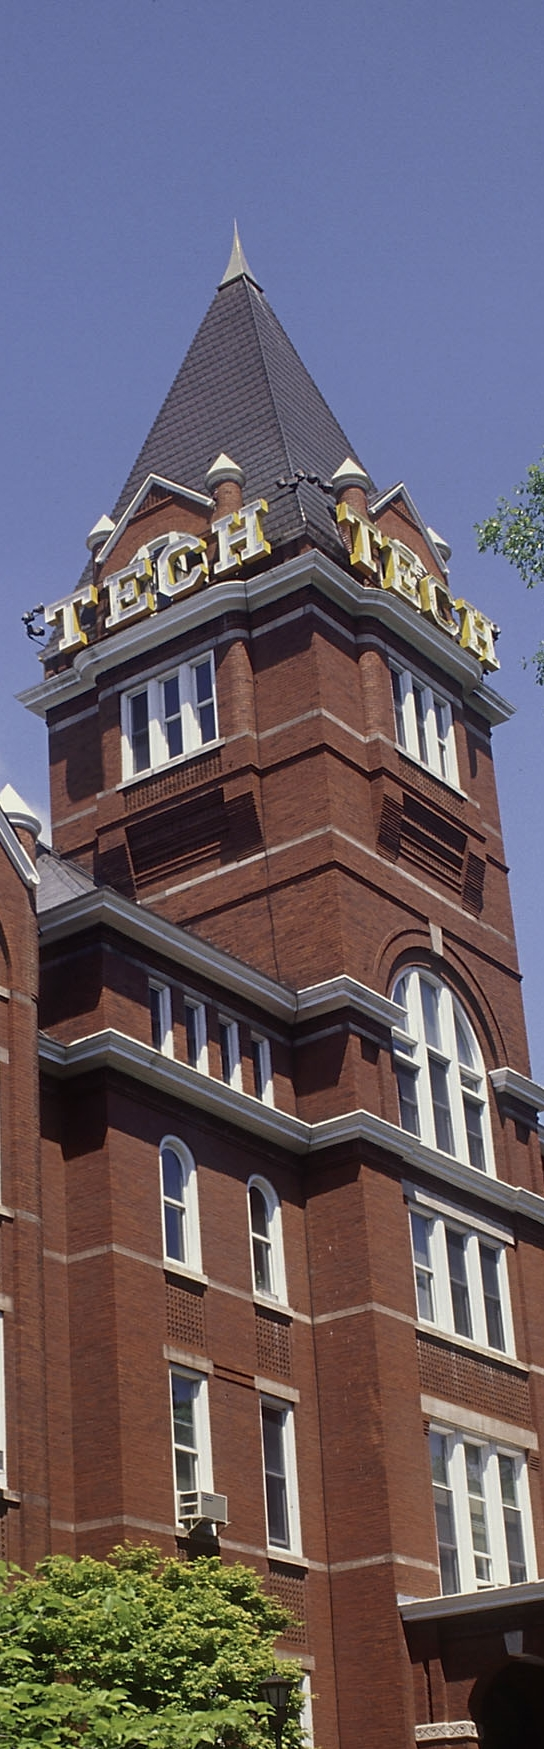
\includegraphics[width=1.25in]{figs/logo_TechTower.jpg}
    	\end{textblock}
    }

%logo tree
    \newcommand{\logoTree}
    {
    	\begin{textblock}{1}(0,0) 
    		\includegraphics[width=1.25in]{figs/logo_tree.jpg}
    	\end{textblock}
    }
%page numbers
    \newcommand{\mypagenum}
    {
    	\begin{textblock}{1}(1,94) 
		{\tiny \color[rgb]{0.2,0.2,1}\insertframenumber} %\insertframenumber,\insertpresentationendpage, \inserttotalframenumber
    	\end{textblock}
    }
%my footnote citation
	\newcommand{\myFootnoteCitation}[2]
	{
		\footnote{\tiny \citeauthor{#1}, \emph{#2}, \citeyear{#1}.}  %\citeauthor{#1}, \citetitle{#1}, #2 \citeyear{#1}.
	}
%my refer to citation
	\newcommand{\mycite}[1]
	{
		\emph{\citeauthor{#1} (\citeyear{#1})}
	}
%my footnote website citation
	\newcommand{\myFootnoteWebsiteCitation}[1]
	{
		\footnote{\tiny \citeauthor{#1}}
	}

\let\thefootnote\relax\footnotetext{Footnotetext without footnote mark}


%section underline
%\newcommand{\tmpsection}[1]{}
%\let\tmpsection=\section
%\renewcommand{\section}[1]{\tmpsection{\underline{#1}}}



%commands
	\newcommand{\likelihood}{p(Z_k| x_k) }						%likelihood
	\newcommand{\prior}{p(x_k)  } 								%prior
	\newcommand{\posterior} {p(x_k| Z_k)}						%posterior
	\newcommand{\prediction} {p(x_k| Z_{k-1})}					%prediction
	\newcommand{\update} {p(x_k|Z_k)}							%update
	\newcommand{\observations} {p(Z_k)}						%observations
	\newcommand{\prevobservations} {p(Z_{k-1})}				%previous observations
	\newcommand{\dxpk} {dx_{k-1}}							%dx_{k-1}
	\newcommand{\ChapKolm}{\int{p(x_k| x_{k-1})p(x_{k-1}|Z_{k-1})} \dxpk} %Chapman Kolmogorov

	%algorithm specific: JPDAF
	\newcommand{\likelihoodJPDAF}{p(Z_k| \chi, m, Z_{k-1}) }		%1. likelihood
	\newcommand{\priorJPDAF}{p(\chi|m, Z^{k-1}} 				%2. prior	
	\newcommand{\observationsJPDAF} {p(Z_k}					%3. observations
	\newcommand{\posteriorJPDAF} {p(\chi| Z_k)}					%4. posterior

%environments
	\newenvironment{changemargin}[2]
	{
	  	\begin{list}{}
		{
			\setlength{\topsep}{0pt}%
			\setlength{\leftmargin}{#1}%
			\setlength{\rightmargin}{#2}%
			\setlength{\listparindent}{\parindent}%
			\setlength{\itemindent}{\parindent}%
			\setlength{\parsep}{\parskip}%
		}
	  	\item[]
		}
		{\end{list}
	}
%figures

%colors
\definecolor{darkgreen}{rgb}{0,0.5,0}

%personal details
	\author{Salman Aslam}
	\institute{Advisor, Dr Christopher Barnes (ECE)\\Co-advisor, Dr Aaron Bobick (CoC)\\Georgia Institute of Technology}
	\date{}

\begin{document}

%####################################################################################################
\title{RVQ \\ extenstive training}
%####################################################################################################
\begin{frame}\logoTechTower
	\author{Salman Aslam}
	\titlepage
\end{frame}

\begin{frame}
\frametitle{Outline}
\logoTechTower\logoCSIPCPL
	\tableofcontents
\end{frame}

%----------------------------------------
\section{RVQ training}
%----------------------------------------
\begin{frame}
\frametitle{Training}
\framesubtitle{}
\logoCSIPCPL\mypagenum
	In the following slides, 
		\begin{itemize}
			\item We train RVQ with all 165 images in the Yale dataset
			\item The goal is to see codebook evolution for different number of templates/stage ($M$) as we vary the target SNR value
			\item Note that varying the target SNR value controls the number of stages
			\item $M$ varies from 2 to 16 ($M=1$ is not allowed)
			\item For every value of $M$, target SNR varies from 0 to 39.8 dB with 0.2 dB increments
		\end{itemize}
\end{frame}

%====================
\subsection{\ \ \ \ \ \ \ \ M: 2}
%====================
\begin{frame}
\frametitle{Training}
\framesubtitle{M: 2 (SNR: 0:0.2:39.8)}
\logoCSIPCPL\mypagenum
	\multiinclude[<+>][format=jpg, start=0, end=199, graphics={height=0.5\textheight}]{figs/RVQ_yaleFaces_dcbk_02_templatesPerStage_padded}
\end{frame}


%====================
\subsection{\ \ \ \ \ \ \ \ M: 3}
%====================
\begin{frame}
\frametitle{Training}
\framesubtitle{M: 3 (SNR: 0:0.2:39.8)}
\logoCSIPCPL\mypagenum
	\multiinclude[<+>][format=jpg, start=0, end=199, graphics={height=0.5\textheight}]{figs/RVQ_yaleFaces_dcbk_03_templatesPerStage_padded}
\end{frame}


%====================
\subsection{\ \ \ \ \ \ \ \ M: 4}
%====================
\begin{frame}
\frametitle{Training}
\framesubtitle{M: 4 (SNR: 0:0.2:39.8)}
\logoCSIPCPL\mypagenum
	\multiinclude[<+>][format=jpg, start=0, end=199, graphics={height=0.5\textheight}]{figs/RVQ_yaleFaces_dcbk_04_templatesPerStage_padded}
\end{frame}



%====================
\subsection{\ \ \ \ \ \ \ \ M: 5}
%====================
\begin{frame}
\frametitle{Training}
\framesubtitle{M: 5 (SNR: 0:0.2:39.8)}
\logoCSIPCPL\mypagenum
	\multiinclude[<+>][format=jpg, start=0, end=199, graphics={height=0.5\textheight}]{figs/RVQ_yaleFaces_dcbk_05_templatesPerStage_padded}
\end{frame}


%====================
\subsection{\ \ \ \ \ \ \ \ M: 6}
%====================
\begin{frame}
\frametitle{Training}
\framesubtitle{M: 6 (SNR: 0:0.2:39.8)}
\logoCSIPCPL\mypagenum
	\multiinclude[<+>][format=jpg, start=0, end=199, graphics={height=0.5\textheight}]{figs/RVQ_yaleFaces_dcbk_06_templatesPerStage_padded}
\end{frame}

%====================
\subsection{\ \ \ \ \ \ \ \ M: 7}
%====================
\begin{frame}
\frametitle{Training}
\framesubtitle{M: 7 (SNR: 0:0.2:39.8)}
\logoCSIPCPL\mypagenum
	\multiinclude[<+>][format=jpg, start=0, end=199, graphics={height=0.5\textheight}]{figs/RVQ_yaleFaces_dcbk_07_templatesPerStage_padded}
\end{frame}



%====================
\subsection{\ \ \ \ \ \ \ \ M: 8}
%====================
\begin{frame}
\frametitle{Training}
\framesubtitle{M: 8 (SNR: 0:0.2:39.8)}
\logoCSIPCPL\mypagenum
	\multiinclude[<+>][format=jpg, start=0, end=199, graphics={height=0.5\textheight}]{figs/RVQ_yaleFaces_dcbk_08_templatesPerStage_padded}
\end{frame}


%====================
\subsection{\ \ \ \ \ \ \ \ M: 9}
%====================
\begin{frame}
\frametitle{Training}
\framesubtitle{M: 9 (SNR: 0:0.2:39.8)}
\logoCSIPCPL\mypagenum
	\multiinclude[<+>][format=jpg, start=0, end=199, graphics={height=0.48\textheight}]{figs/RVQ_yaleFaces_dcbk_09_templatesPerStage_padded}
\end{frame}


%====================
\subsection{\ \ \ \ \ \ \ \ M: 10}
%====================
\begin{frame}
\frametitle{Training}
\framesubtitle{M: 10 (SNR: 0:0.2:39.8)}
\logoCSIPCPL\mypagenum
	\multiinclude[<+>][format=jpg, start=0, end=199, graphics={height=0.48\textheight}]{figs/RVQ_yaleFaces_dcbk_10_templatesPerStage_padded}
\end{frame}


%====================
\subsection{\ \ \ \ \ \ \ \ M: 11}
%====================
\begin{frame}
\frametitle{Training}
\framesubtitle{M: 11 (SNR: 0:0.2:39.8)}
\logoCSIPCPL\mypagenum
	\multiinclude[<+>][format=jpg, start=0, end=199, graphics={height=0.48\textheight}]{figs/RVQ_yaleFaces_dcbk_11_templatesPerStage_padded}
\end{frame}


%====================
\subsection{\ \ \ \ \ \ \ \ M: 12}
%====================
\begin{frame}
\frametitle{Training}
\framesubtitle{M: 12 (SNR: 0:0.2:39.8)}
\logoCSIPCPL\mypagenum
	\multiinclude[<+>][format=jpg, start=0, end=199, graphics={height=0.48\textheight}]{figs/RVQ_yaleFaces_dcbk_12_templatesPerStage_padded}
\end{frame}


%====================
\subsection{\ \ \ \ \ \ \ \ M: 13}
%====================
\begin{frame}
\frametitle{Training}
\framesubtitle{M: 13 (SNR: 0:0.2:39.8)}
\logoCSIPCPL\mypagenum
	\multiinclude[<+>][format=jpg, start=0, end=199, graphics={height=0.48\textheight}]{figs/RVQ_yaleFaces_dcbk_13_templatesPerStage_padded}
\end{frame}


%====================
\subsection{\ \ \ \ \ \ \ \ M: 14}
%====================
\begin{frame}
\frametitle{Training}
\framesubtitle{M: 14 (SNR: 0:0.2:39.8)}
\logoCSIPCPL\mypagenum
	\multiinclude[<+>][format=jpg, start=0, end=199, graphics={height=0.48\textheight}]{figs/RVQ_yaleFaces_dcbk_14_templatesPerStage_padded}
\end{frame}


%====================
\subsection{\ \ \ \ \ \ \ \ M: 15}
%====================
\begin{frame}
\frametitle{Training}
\framesubtitle{M: 15 (SNR: 0:0.2:39.8)}
\logoCSIPCPL\mypagenum
	\multiinclude[<+>][format=jpg, start=0, end=199, graphics={height=0.48\textheight}]{figs/RVQ_yaleFaces_dcbk_15_templatesPerStage_padded}
\end{frame}


%====================
\subsection{\ \ \ \ \ \ \ \ M: 16}
%====================
\begin{frame}
\frametitle{Training}
\framesubtitle{M: 16 (SNR: 0:0.2:39.8)}
\logoCSIPCPL\mypagenum
	\multiinclude[<+>][format=jpg, start=0, end=1, graphics={height=0.48\textheight}]{figs/RVQ_yaleFaces_dcbk_16_templatesPerStage_padded}
\end{frame}


%####################################################################################################
%####################################################################################################
%\bibliographystyle{ieee}
%\bibliography{c:/salman/work/writing/MyCitations}
\end{document}
%####################################################################################################

%####################################################################################################
